\documentclass[tikz,border=10pt]{standalone}
\usetikzlibrary{positioning, mindmap}

\definecolor{morange}{RGB}{255,127,14}
\definecolor{mblue}{RGB}{31,119,180}
\definecolor{mred}{RGB}{214,39,40}
\definecolor{mpurple}{RGB}{148,103,189}
\definecolor{mgreen}{RGB}{44,160,44}

\begin{document}
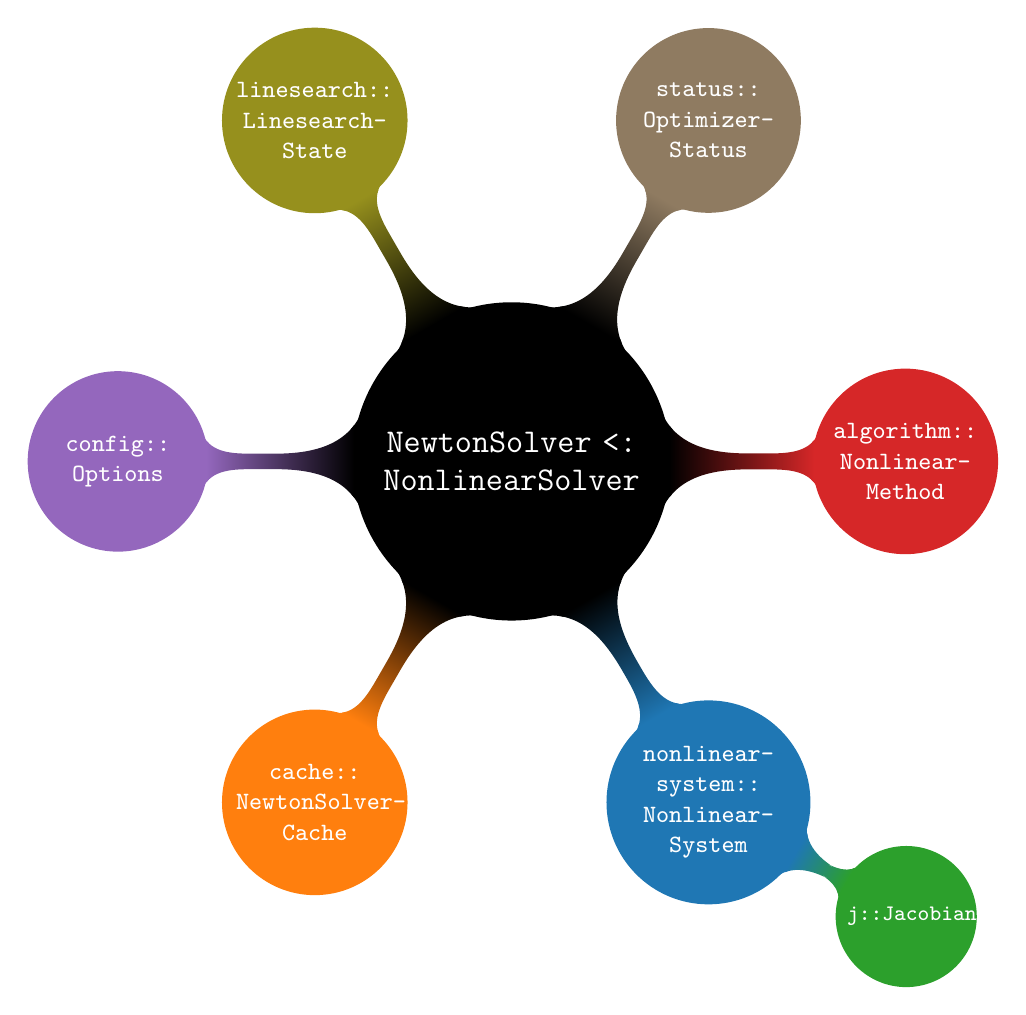
\begin{tikzpicture}
  \path[mindmap,concept color=black,text=white]
    node[concept] {\texttt{NewtonSolver <: \\NonlinearSolver}}
    [clockwise from=0]
    % note that `sibling angle' can only be defined in
    % `level 1 concept/.append style={}'
    % note that the `concept color' is passed to the `child'(!)
    child[concept color=mred] {node[concept] {\texttt{algorithm::\\Nonlinear-\\Method}} }
    child[concept color=mblue] {node[concept] {\texttt{nonlinear-\\system::\\Nonlinear-\\System}} [clockwise from=-30] child[concept color=mgreen] { node[concept] {\texttt{j::Jacobian}}}}
    child[concept color=morange] {node[concept] {\texttt{cache::\\NewtonSolver-\\Cache}} }
    child[concept color=mpurple] {node[concept] {\texttt{config::\\Options}}}
    child[concept color=morange!50!mgreen] {node[concept] {\texttt{linesearch::\\Linesearch-\\State}}}
    child[concept color=morange!50!mblue] {node[concept] {\texttt{status::\\Optimizer-\\Status}}};
\end{tikzpicture}
\end{document}